\section{Desarrollo}

El desarrollo se dividió en dos secciones:
\begin{itemize}
    \item Análisis de programa
    \item Análisis electrónico
\end{itemize}

A continuación, se muestra una breve descripción de los resultados a los que se llegaron en este laboratorio, así como a nivel de hardware, y software.

\subsection{Análisis de programa}
La descripción de cada subrutina diseñada para este laboratorio se encuentra en la documentación del código fuente, así como los diagramas de llamado a funciones generados por Doxygen. 

\subsection{Análisis electrónico}

A continuación, se muestra una captura de pantalla que contiene una lectura de tensión del pin conectado al pulsador, y una lectura de corriente fluyendo en los LEDs. 

\begin{figure}[!h]
    \centering
    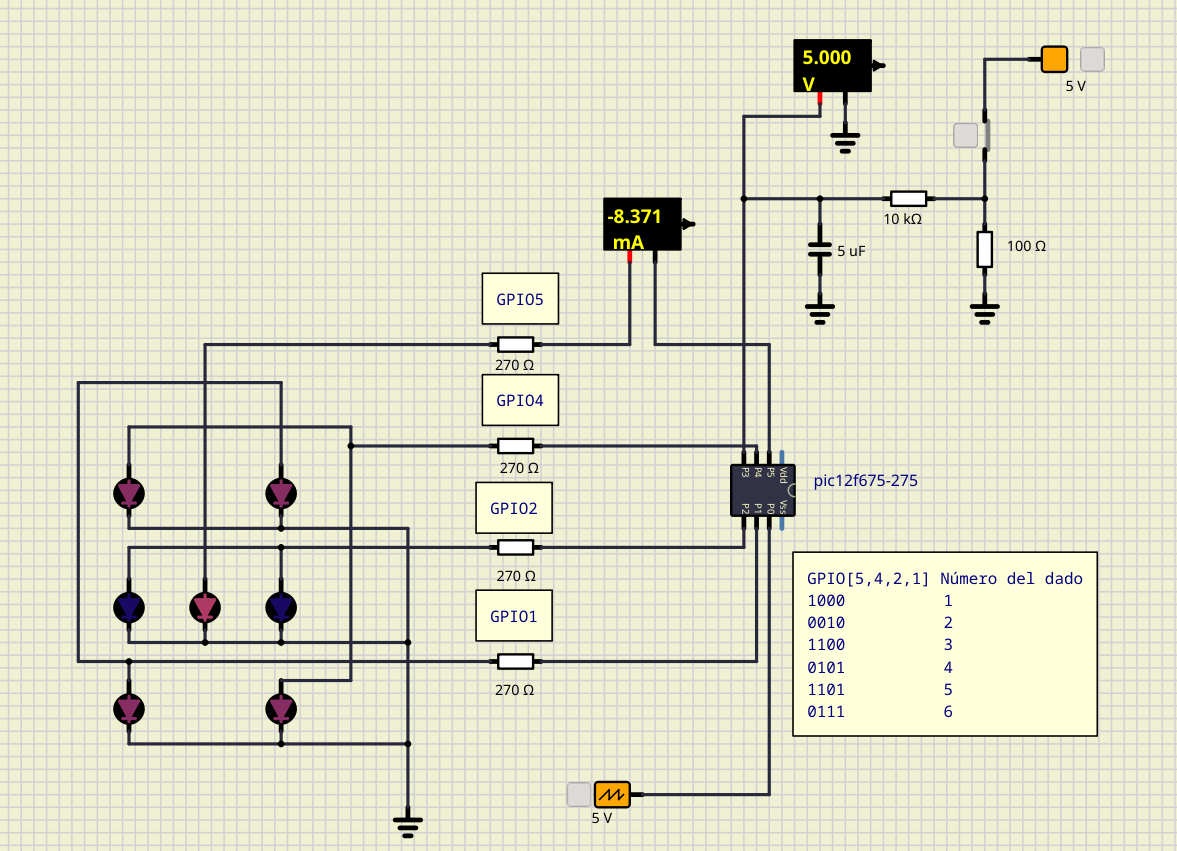
\includegraphics[width = 0.8\linewidth]{imagenes/fig12.png}
    \caption{Lecturas analógicas de parámetros del circuito del simulador de dado}
    \label{fig13}
\end{figure}

Como se puede ver en la figura anterior, la tensión al pulsar el botón es la esperada. Ademaś de esto, la corriente que fluye por los LEDs cuando uno de estos es encendido por medio de un GPIO es menor a \SI{10}{mA}, lo cual confirma que el diseño de $R _{LED}$ es correcto.
Al tocar el pulsador varias veces, se percibe que el número mostrado en la cara del dado no sigue un patrón aparente, gracias a la lectura del pin flotante del $\mu C$. Debido a esto, se asegura que el dado efectivamente muestra números aleatorios entre 1 y 6 en la cara del dado.


